\documentclass[10pt]{article}
\usepackage{tikz}
\usetikzlibrary{shapes.misc}
\usepackage[margin=0cm]{geometry}
\pagestyle{empty}
\tikzstyle{every node}=[cross out, draw, red]

\begin{document}

\vspace*{\fill}
\begin{center}
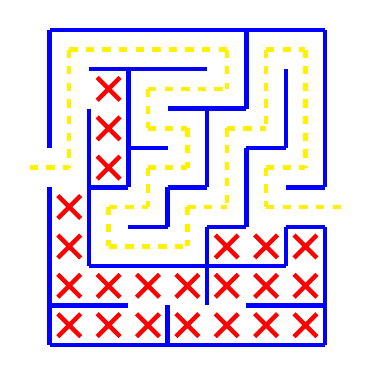
\begin{tikzpicture}[x=0.5cm, y=-0.5cm, ultra thick, blue]
% Walls
    \draw (0,0) -- (7,0);
    \draw (1,1) -- (4,1);
    \draw (3,2) -- (5,2);
    \draw (2,3) -- (3,3);
    \draw (5,3) -- (6,3);
    \draw (1,4) -- (2,4);
    \draw (3,4) -- (4,4);
    \draw (6,4) -- (7,4);
    \draw (2,5) -- (3,5);
    \draw (4,5) -- (5,5);
    \draw (6,5) -- (7,5);
    \draw (1,6) -- (6,6);
    \draw (0,7) -- (2,7);
    \draw (5,7) -- (7,7);
    \draw (0,8) -- (7,8);
    \draw (0,0) -- (0,3);
    \draw (0,4) -- (0,8);
    \draw (1,2) -- (1,6);
    \draw (2,1) -- (2,4);
    \draw (3,4) -- (3,5);
    \draw (3,7) -- (3,8);
    \draw (4,2) -- (4,4);
    \draw (4,5) -- (4,7);
    \draw (5,0) -- (5,2);
    \draw (5,3) -- (5,5);
    \draw (6,1) -- (6,3);
    \draw (6,5) -- (6,6);
    \draw (7,0) -- (7,4);
    \draw (7,5) -- (7,8);
% Pillars
% Inner points in accessible cul-de-sacs
    \node at (1.5,1.5) {};
    \node at (1.5,2.5) {};
    \node at (1.5,3.5) {};
    \node at (0.5,4.5) {};
    \node at (0.5,5.5) {};
    \node at (4.5,5.5) {};
    \node at (5.5,5.5) {};
    \node at (6.5,5.5) {};
    \node at (0.5,6.5) {};
    \node at (1.5,6.5) {};
    \node at (2.5,6.5) {};
    \node at (3.5,6.5) {};
    \node at (4.5,6.5) {};
    \node at (5.5,6.5) {};
    \node at (6.5,6.5) {};
    \node at (0.5,7.5) {};
    \node at (1.5,7.5) {};
    \node at (2.5,7.5) {};
    \node at (3.5,7.5) {};
    \node at (4.5,7.5) {};
    \node at (5.5,7.5) {};
    \node at (6.5,7.5) {};
% Entry-exit paths without intersections
    \draw[dashed, yellow] (0.5,0.5) -- (4.5,0.5);
    \draw[dashed, yellow] (5.5,0.5) -- (6.5,0.5);
    \draw[dashed, yellow] (2.5,1.5) -- (4.5,1.5);
    \draw[dashed, yellow] (2.5,2.5) -- (3.5,2.5);
    \draw[dashed, yellow] (4.5,2.5) -- (5.5,2.5);
    \draw[dashed, yellow] (-0.5,3.5) -- (0.5,3.5);
    \draw[dashed, yellow] (2.5,3.5) -- (3.5,3.5);
    \draw[dashed, yellow] (5.5,3.5) -- (6.5,3.5);
    \draw[dashed, yellow] (1.5,4.5) -- (2.5,4.5);
    \draw[dashed, yellow] (3.5,4.5) -- (4.5,4.5);
    \draw[dashed, yellow] (5.5,4.5) -- (7.5,4.5);
    \draw[dashed, yellow] (1.5,5.5) -- (3.5,5.5);
    \draw[dashed, yellow] (0.5,0.5) -- (0.5,3.5);
    \draw[dashed, yellow] (1.5,4.5) -- (1.5,5.5);
    \draw[dashed, yellow] (2.5,1.5) -- (2.5,2.5);
    \draw[dashed, yellow] (2.5,3.5) -- (2.5,4.5);
    \draw[dashed, yellow] (3.5,2.5) -- (3.5,3.5);
    \draw[dashed, yellow] (3.5,4.5) -- (3.5,5.5);
    \draw[dashed, yellow] (4.5,0.5) -- (4.5,1.5);
    \draw[dashed, yellow] (4.5,2.5) -- (4.5,4.5);
    \draw[dashed, yellow] (5.5,0.5) -- (5.5,2.5);
    \draw[dashed, yellow] (5.5,3.5) -- (5.5,4.5);
    \draw[dashed, yellow] (6.5,0.5) -- (6.5,3.5);
\end{tikzpicture}
\end{center}
\vspace*{\fill}

\end{document}
